\chapter{I-Mode Pedestal Scalings}\label{ch:ImodePedestal}

The I-mode \cite{Whyte2010,Hubbard2011}, introduced in \cref{sec:hcr_imode}, is a novel high-performance regime pioneered on Alcator C-Mod.  I-mode is unique in that it appears to decouple energy and particle transport, forming a steep temperature pedestal with H-mode levels of energy confinement without the accompanying density pedestal or suppression of particle transport found in conventional H-modes.  I-mode exhibits several highly attractive properties for a putative reactor regime:

\begin{enumerate}
 \item Due to the lack of particle transport suppression (as is found in H-modes), the I-mode retains L-mode-like impurity confinement times, avoiding the accumulation of deleterious impurities in the plasma, including those from high-$Z$ metal plasma-facing components necessary for reactor operation \cite{Loarte2007}.  This ensures stationary operation without the need for ELMs or continuous fluctuations in the edge to provide the necessary relaxation of the particle confinement.
 \item I-mode appears to be naturally stable against large ELMs, avoiding excessive pulsed heat loading to plasma-facing components without externally-applied engineering controls (described in \cref{subsec:hcr_elmy_control}).
 \item Energy confinement in I-mode appears to exhibit little to know degradation with input heating power, in contrast to that found in ELMy H-mode ($\tau_E \sim P^{-0.7}$ from the ITER98y2 analysis \cite{ITER1999}), scaling quite favorably to reactor-scale devices.
\end{enumerate}

\begin{figure}[t]
 \pushtooutside
 \fcapside[60mm]{\caption[L-mode and I-mode edge profiles from a single discharge.]{L-mode (black) and I-mode (red) edge profiles from a single discharge.  I-mode maintains a comparable density profile (particularly, there is no change in $\nabla n_e$ or formation of a density pedestal), while forming an H-mode-like temperature pedestal.  \note{rescale, add detail?  repeat fig. 2.6?}}
 \label{fig:imode_pedestal}}{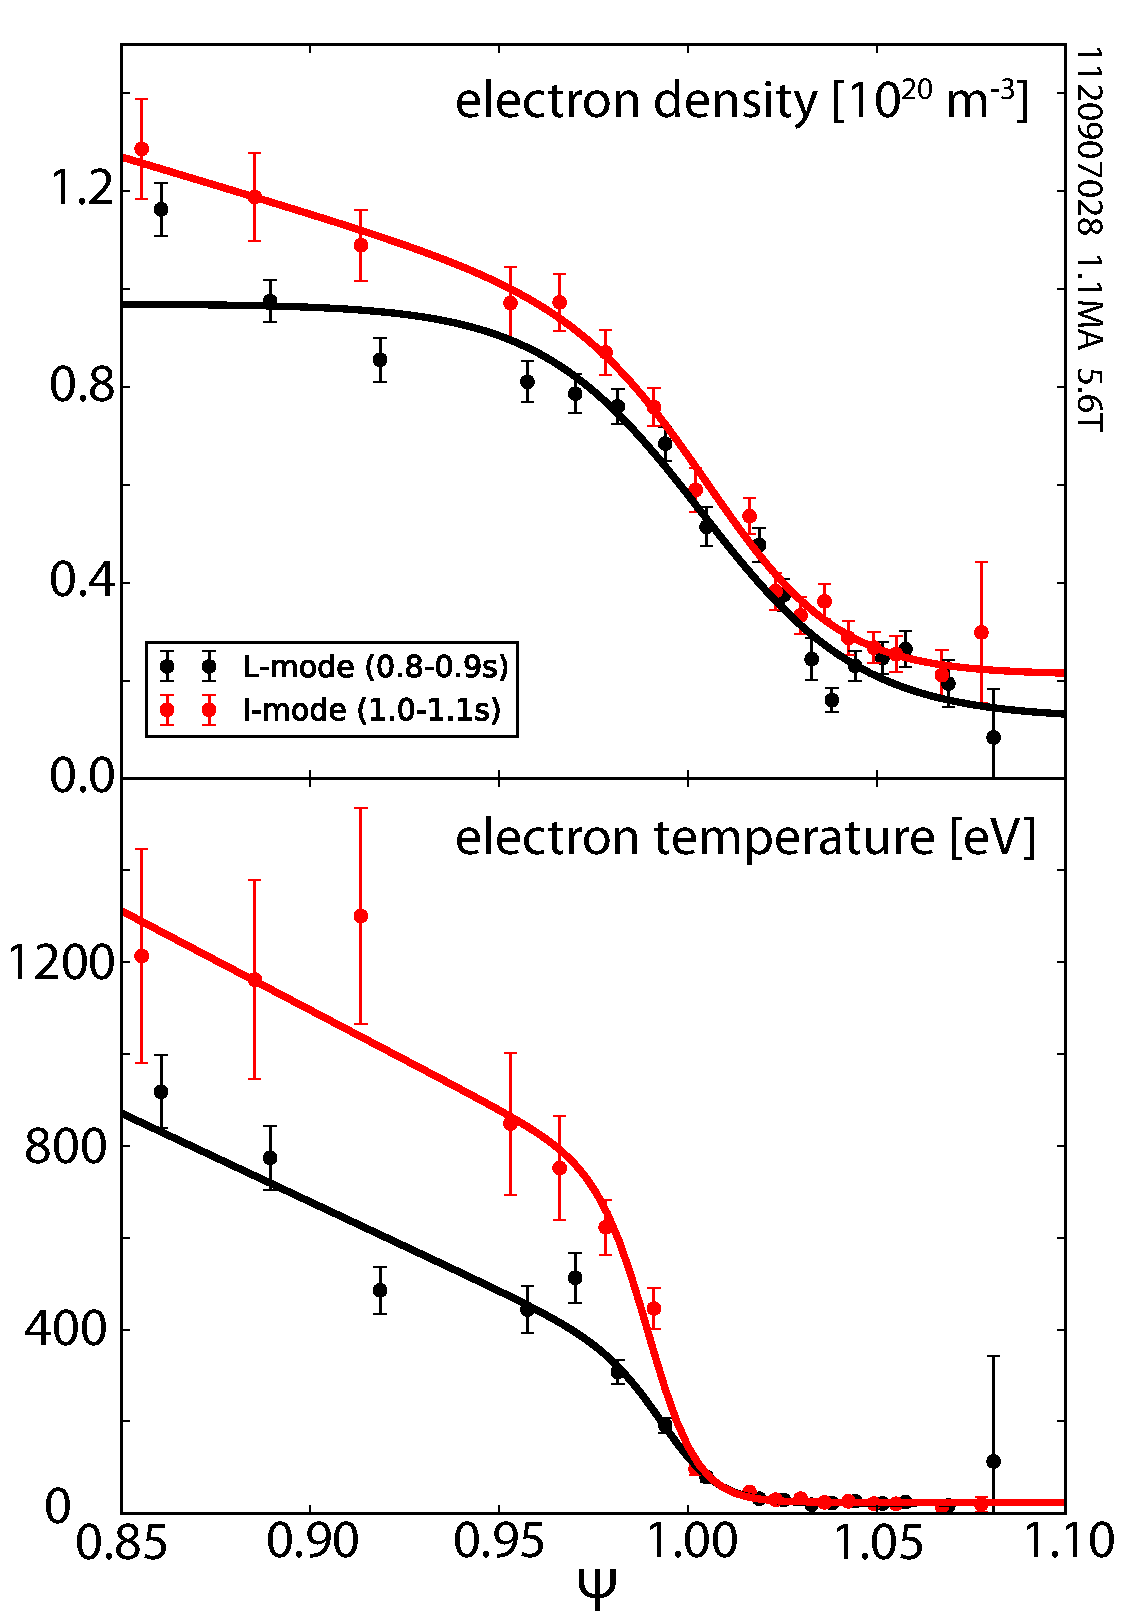
\includegraphics[width=100mm]{graphics/IModePedestal/1120907028_dens_temp.pdf}}
\end{figure}

A firm understanding of the pedestal is essential for the extrapolation of any high-performance regime to ITER- and reactor-scale devices.  The pedestal height sets a strong constraint on core temperature and pressure -- and therefore overall fusion performance -- both by acting as a boundary condition for the plasma profiles, and by supporting steeper core temperature gradients due to profile stiffness \cite{Kinsey2011,Hubbard1998}.  Moreover, the pedestal structure, particularly the steep gradients in density, temperature, and/or pressure, determines stability of the plasma against large, deleterious ELMs (see \cref{sec:mod_pb}).  In this chapter, we review empirical observations of the pedestal in I-mode from a recent series of dedicated experiments, with a focus on high-resolution pedestal profile measurements across a range of plasma parameters.  Through this, we examine trends in I-mode pedestal behavior, and their impact on global behavior and performance in I-mode, and possible extrapolations to larger devices\gnote{be more specific... maybe?}.\nicesectionending

\section{Access and Experimental Setup}\label{sec:imode_setup}

All data presented here was taken on the Alcator C-Mod tokamak, described in \cref{sec:intro_cmod}.  As described in \cref{subsec:hcr_imode_access}, I-mode access hinges primarily on operation with the ion $\nabla B$ drift (\cref{eq:gradbdrift}) directed away from the primary X-point in the plasma (the ``unfavorable $\nabla B$ drift'' configuration).  Within this requirement, though, I-mode access is fairly robust, with steady I-modes sustained in a variety of shapes -- both USN with standard field, and LSN shapes with reversed field to achieve the desired $\nabla B$ drift direction (in the latter case, the plasma current is reversed as well to preserve field helicity) -- and edge-current profiles, and at low-to-moderate collisionality (\cref{eq:nustar}).  The attainable range in $q_{95}$ and $\nu^*_{95}$ is shown in \cref{fig:imode_q_nustar}.

\begin{figure}[h]
 \pushtooutside
 \fcapside[60mm]{\caption[I-mode edge safety collisionality and safety factor.]{Range in edge collisionality $\nu^*_{95}$ and $q_{95}$ over which I-modes have been accessed.  Notably, I-mode operation is naturally favored near ITER targets for these parameters.  The subset of this data prepared with high-resolution pedestal profiles, herein termed the ``pedestal database'', is also highlighted.}\label{fig:imode_q_nustar}}{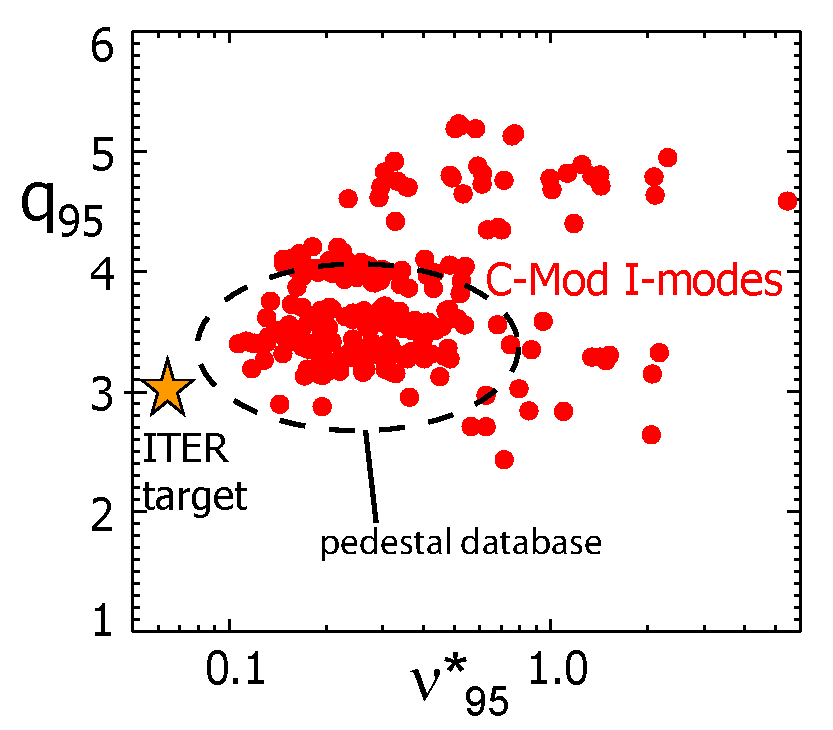
\includegraphics[width=100mm]{graphics/IModePedestal/q95_vs_nustar_2012_Imodeonly.pdf}}
\end{figure}

\begin{figure}[h]
 \pushtooutside
 \fcapside[60mm]{\caption[Density and power range for I-mode access]{Line-averaged density and loss power range for USN and LSN I-modes, illustrating $\sim 2 \times P_{L-I}$ range for $1-\SI{1.2}{\mega\ampere}$, $5-\SI{6}{\tesla}$ I-modes.  USN shapes are forward-field and LSN-shapes are reversed field, such that all I-modes shown are in the unfavorable drift configuration.  \note{swap for plot showing only high-res database, or merge?}}}{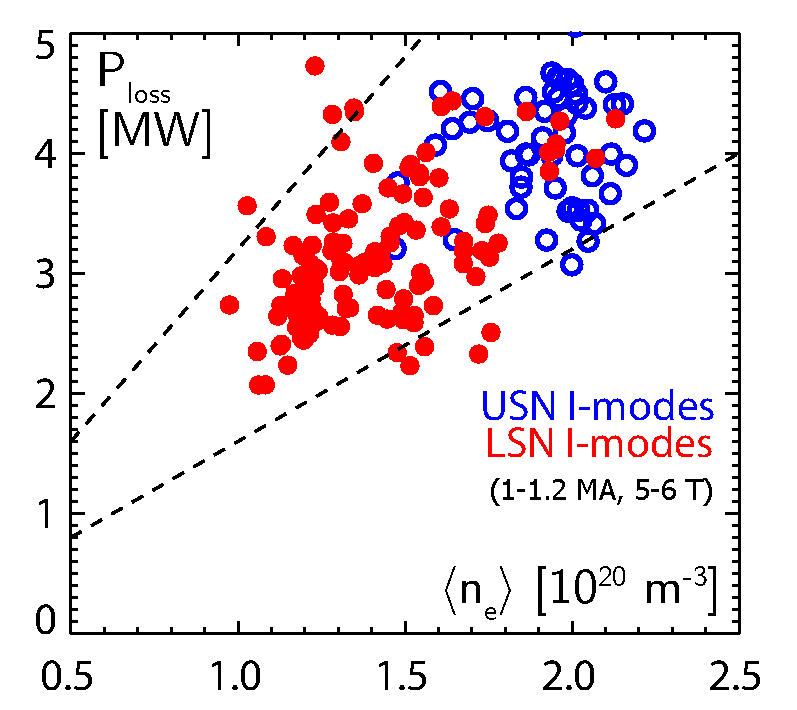
\includegraphics[width=100mm]{graphics/IModePedestal/Ploss_nebar_2013.pdf}}
\end{figure}

\nicesectionending

\section{Pedestal Responses}\label{sec:imode_height}

\subsection{Pedestal Temperature}\label{subsec:imode_temp}

\subsection{Pedestal Response to Fueling}\label{subsec:imode_fueling}

\begin{figure}[ht]
 \pushtooutside
 \fcapside[60mm]{\caption[Density and temperature pedestals at matched current and field with varying fueling and heating power -- matched $P_{net}/\overline{n}_e$ maintains the $T_e$ pedestal.]{Density and temperature pedestals at matched current, field, and shaping, with varying fueling and heating power levels.  The three discharges are fueled to $\overline{n}_e$ of $\num{1.0}$ (black), $\num{1.3}$ (blue), and $\SI{1.7e20}{\per\meter\cubed}$ (red) respectively, with heating powers of $\num{2.75}$, $\num{3.65}$, and $\SI{4.10}{\mega\watt}$ to maintain matched $P_{net}/\overline{n}_e \sim 2.4-2.7$.  The constant power-per-particle maintains matched temperature pedestals across the fueling range, indicative of the independent control of pedestal $n_e$ and $T_e$ available in I-mode.}\label{fig:imode_fuelingprofiles}}{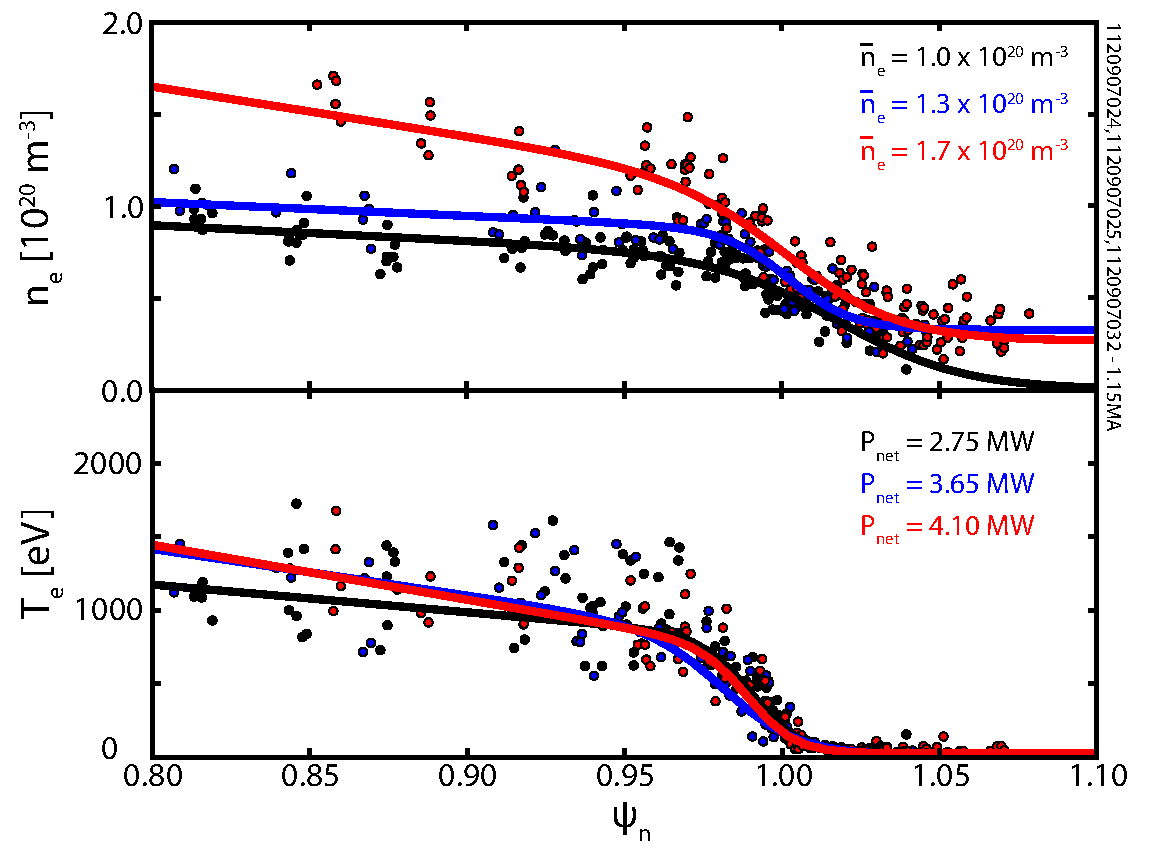
\includegraphics[width=100mm]{graphics/IModePedestal/fuelingprofiles.pdf}}
\end{figure}

\subsection{Pressure Pedestal Scalings and Performance}\label{subsec:imode_pres}

\nicesectionending

\section{Pedestal Widths}\label{sec:imode_width}

\begin{figure}
 \pushtooutside
 \fcapside[60mm]{\caption[Pedestal width vs. poloidal beta in I-mode and ELMy H-mode.]{Pedestal width versus poloidal beta in I-mode and ELMy H-mode.  ELMy H-modes lie on the $\Delta_\psi \sim \beta_{p,ped}^{1/2}$ line predicted for KBM-limited pedestals (see \cref{subsec:elmy_eped_width}).  I-mode shows no scaling of the pedestal width with $\beta_p$, and exhibits pedestals consistently wider than predicted for comparable ELM-limited pedestals.}\label{fig:imode_wid_betapol}}{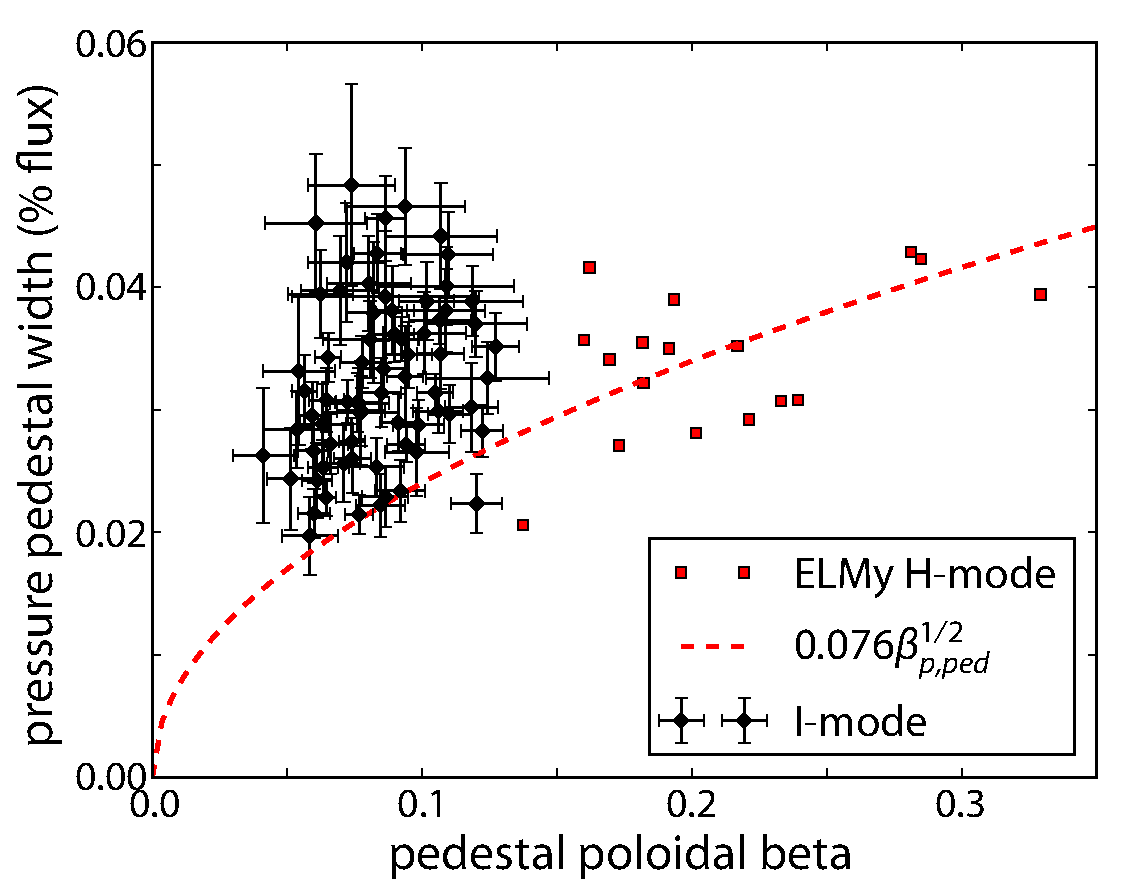
\includegraphics[width=100mm]{graphics/IModePedestal/wid_betapol.pdf}}
\end{figure}

\nicesectionending

\section{Global Behavior, Performance, \& Confinement}\label{sec:imode_confinement}

\begin{table*}
 \pushtooutside
 \ttabbox{\caption[Parameters for power-law scalings of I-mode energy confinement time.]{Parameters for power-law scalings of the I-mode energy confinement time $\tau_E$, along with $R^2$ coefficients of determination for the fit.  Blank entries indicate parameters that were omitted from that fit.  Note that fit \#5 utilized a fixed $R^2 \sqrt{\varepsilon}$ size dependence rather than taking the size to be a free fitting parameter.  Parameters are in the given units: $I_p$ in $\si{\mega\ampere}$, $B_T$ in $\si{\tesla}$, $\overline{n}_e$ in $\SI{e20}{\per\meter\cubed}$, $R$ in $\si{\meter}$, and $P_{loss}$ in $\si{\mega\watt}$.  Elongation $\kappa$ and aspect ratio $\varepsilon$ are dimensionless.}\label{tab:imode_confinement}}{
 \begin{tabular}{cccccc}
  \toprule
  & \#1 & \#2 & \#3 & \#4 & \#5 \\
  \midrule
  $C$ & $0.040 \pm 0.066$ & $0.007 \pm 0.002$ & $0.014 \pm 0.002$ & $0.014 \pm 0.002$ & $0.056 \pm 0.008$ \\
  $I_p$ & $0.686 \pm 0.074$ & $0.696 \pm 0.073$ & $0.685 \pm 0.076$ & $0.692 \pm 0.073$ & $0.676 \pm 0.077$ \\
  $B_T$ & $0.698 \pm 0.075$ & $0.697 \pm 0.071$ & $0.768 \pm 0.072$ & $0.773 \pm 0.071$ & $0.767 \pm 0.072$ \\
  $\overline{n}_e$ & $-0.077 \pm 0.055$ & $-0.050 \pm 0.048$ & $0.017 \pm 0.048$ & & $0.006 \pm 0.048$ \\
  $R$ & $4.219 \pm 4.623$ & & & & $2^*$ \\
  $\varepsilon$ & $0.127 \pm 1.144$ & & & & $0.5^*$ \\
  $\kappa$ & $1.686 \pm 0.398$ & $1.501 \pm 0.350$ & & & \\
  $P_{loss}$ & $-0.197 \pm 0.048$ & $-0.220 \pm 0.043$ & $-0.286 \pm 0.042$ & $-0.281 \pm 0.039$ & $-0.275 \pm 0.042$ \\
  $R^2$ & $0.713$ & $0.711$ & $0.685$ & $0.684$ & $0.683$ \\
  \bottomrule
 \end{tabular}
 }
\end{table*}

\begin{figure}
 \pushtooutside
 \fcapside[60mm]{\caption[Power-law fit to I-mode $\tau_E$ with full parameter set.]{Power-law fit for I-mode energy confinement time $\tau_E$, fitted using the full ITER98y2 parameter set (fit \#1 in \cref{tab:imode_confinement}).  Both the high-resolution pedestal database and older reversed-field LSN and forward-field USN I-mode databases are used.  While the fit is generally good, lack of variation in certain parameters -- particularly the size parameters $R$ and $\varepsilon$ (as expected for a single-machine scaling), and elongation $\kappa$ mean that the true variation with these parameters is not accurately captured.  However, the expected weak degradation of $\tau_E$ with heating power is captured.}\label{fig:imode_tauE_1}}{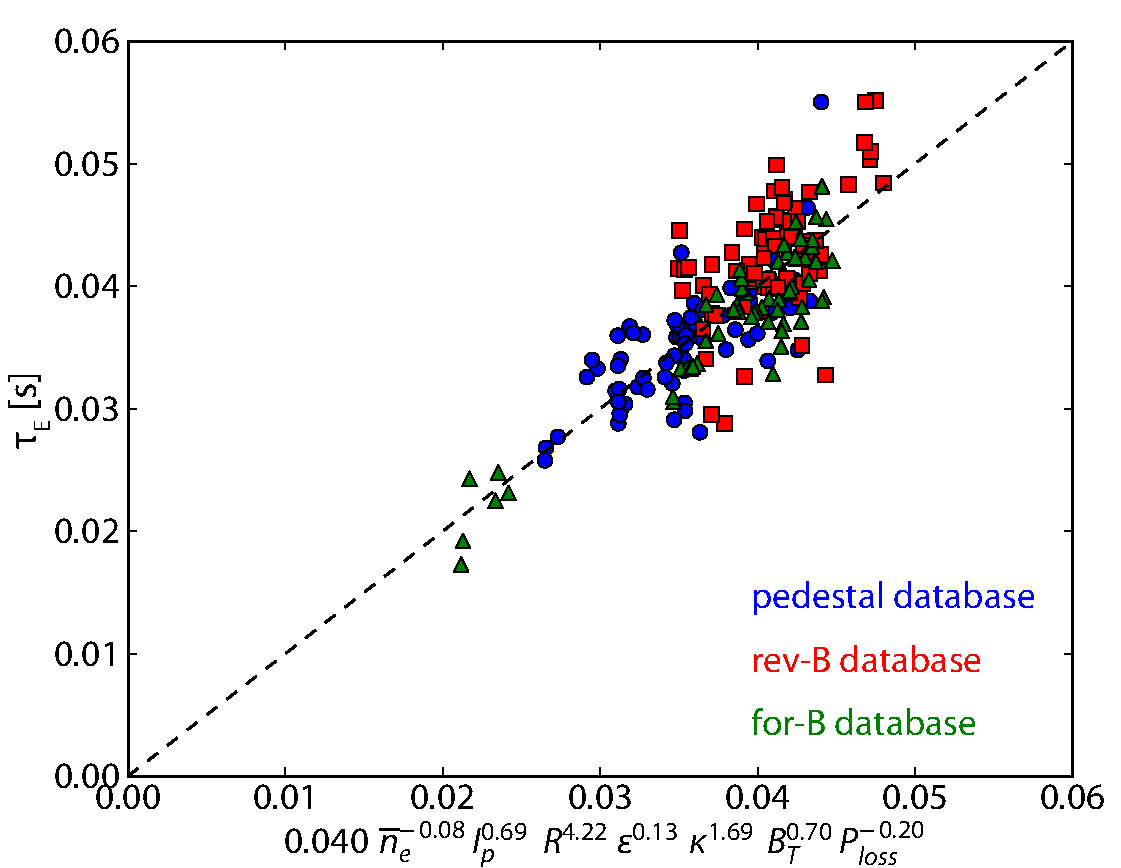
\includegraphics[width=100mm]{graphics/IModePedestal/tauE_1_Ploss_sep.pdf}}
\end{figure}

\begin{figure}
 \pushtooutside
 \fcapside[60mm]{\caption[Power-law fit to I-mode $\tau_E$, with poorly-fitted parameters excluded.]{Power-law fit for I-mode energy confinement time $\tau_E$, fitted with the size parameters $R$ and $\varepsilon$, and elongation $\kappa$ excluded due to the lack of variation in these variables in the available data (fit \#3 in \cref{tab:imode_confinement}).  Both the high-resolution pedestal database and older reversed-field LSN and forward-field USN I-mode databases are used.}\label{fig:imode_tauE_3}}{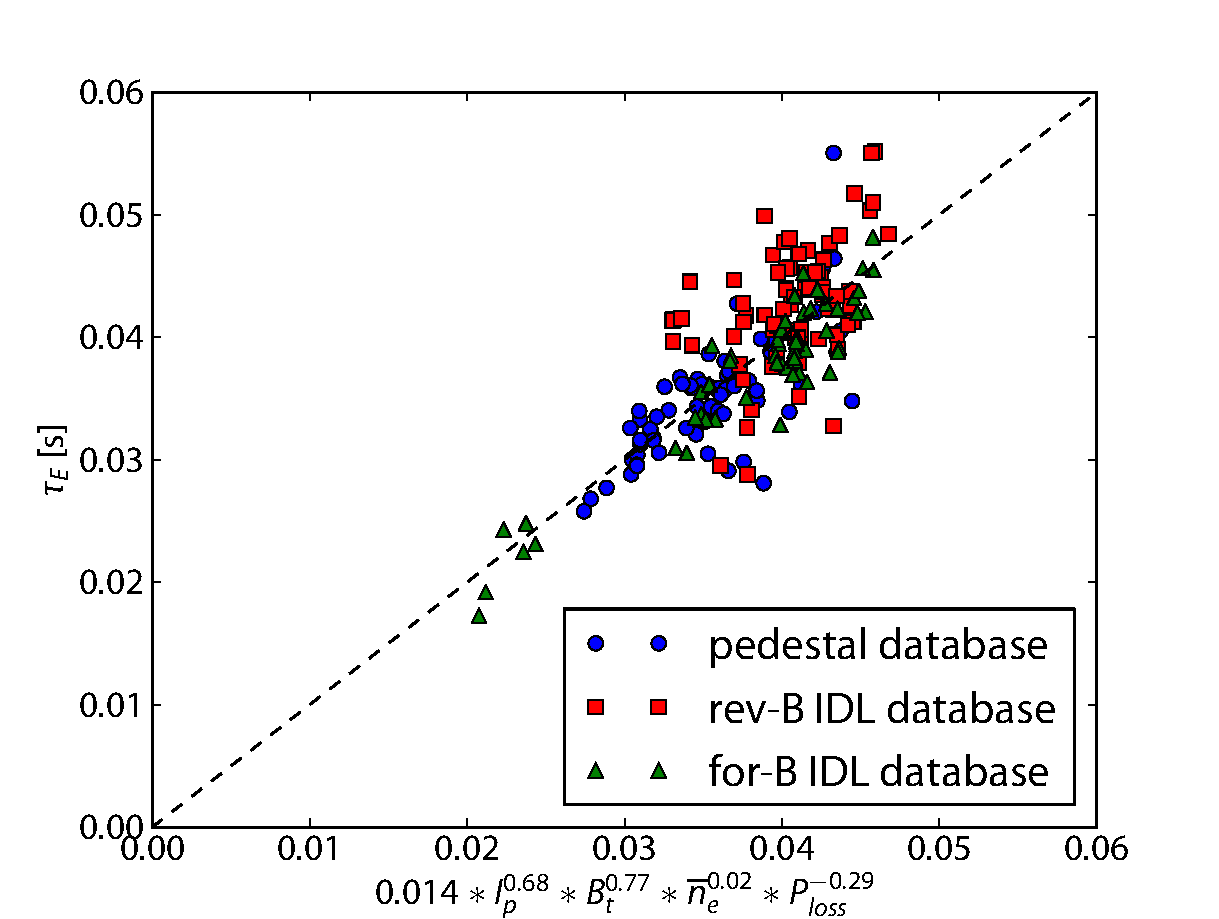
\includegraphics[width=100mm]{graphics/IModePedestal/tauE_3_Ploss_sep.pdf}}
\end{figure}

\begin{figure}
 \pushtooutside
 \fcapside[60mm]{\caption[Power-law fit to I-mode $\tau_E$, with fixed $R^2 \sqrt{\varepsilon}$ size scaling.]{Power-law fit to I-mode energy confinement time $\tau_E$, with the \emph{ansatz} of an $R^2 \sqrt{\varepsilon}$ size scaling fixed (fit \#5 in \cref{tab:imode_confinement}).  Both the high-resolution pedestal database and older reversed-field LSN and forward-field USN I-mode databases are used.  Note the expected weak degradation of $\tau_E$ with heating power.}\label{fig:imode_tauE_6}}{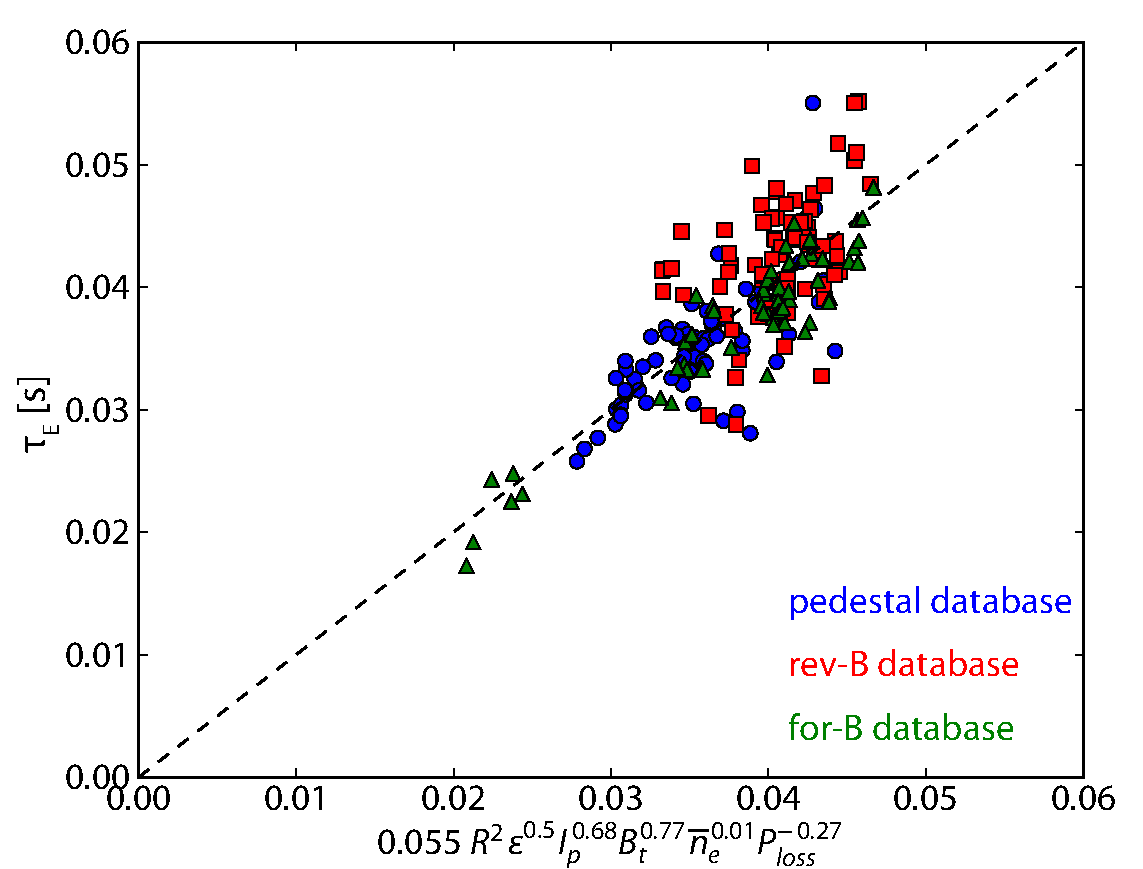
\includegraphics[width=100mm]{graphics/IModePedestal/tauE_6_Ploss_sep.pdf}}
\end{figure}

\begin{figure}
 \pushtooutside
 \fcapside[60mm]{\caption[Power-law fit to I-mode $\tau_E$ extrapolated to larger devices.]{Modeled energy confinement time $\tau_E$ with the fixed $R^2 \sqrt{\varepsilon}$ size scaling (fit \#5 in \cref{tab:imode_confinement}, extrapolated to DIII-D, ASDEX Upgrade, JET, and ITER.  Modeled energy confinement times are competitive with H-modes, both the measured $\tau_E$ for existing machines and the expected ITER98y2 prediction for ITER H-modes.}\label{fig:imode_tauE_extrap}}{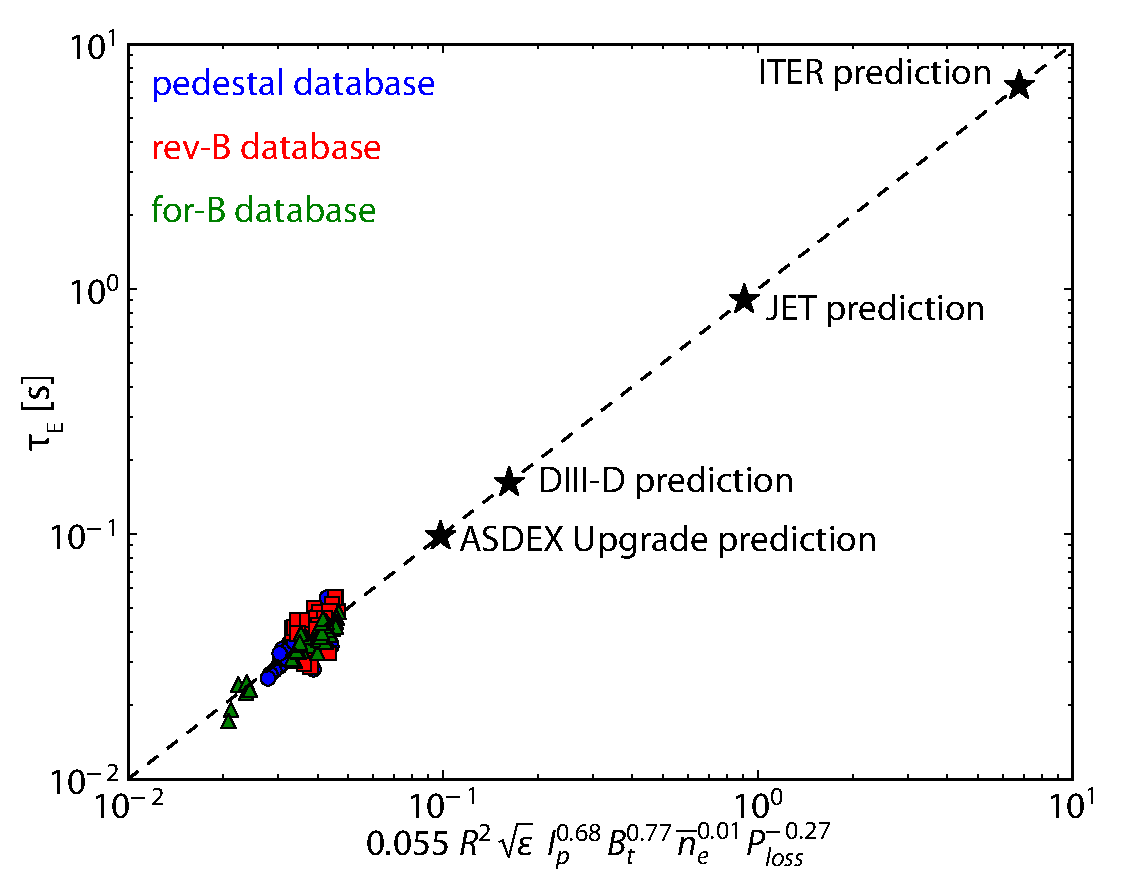
\includegraphics[width=100mm]{graphics/IModePedestal/tauE_6_Ploss_extrap.pdf}}
\end{figure}

\section{Fluctuation Characterization}\label{sec:imode_fluct}

\nicechapterending

\bibliographystyle{../plainurl}
\bibliography{../references}